\documentclass[aspectratio=169]{beamer}
\usepackage[utf8]{inputenc}
\usepackage[T1]{fontenc}
\usepackage{tikz}
\usepackage{hyperref}

\usepackage{pgfpages}
\setbeameroption{show notes on second screen}
% \pgfpagesuselayout{2 on 1}[a4paper,border shrink=10mm]

\usetheme[darkmode, nofooterlogo]{pureminimalistic}
% \renewcommand{\pageword}{}
\renewcommand{\logotitle}{}
\renewcommand{\logoheader}{}
\renewcommand{\logofooter}{}
\usepackage[backend=biber, doi=false, maxbibnames=2, maxcitenames=2, style=numeric, sorting=none, url=false, eprint=false]{biblatex}
\addbibresource{bibliography.bib}
\usepackage{appendixnumberbeamer}
\renewcommand{\appendixname}{\texorpdfstring{\translate{appendix}}{appendix}}

\title[Debugging of RxJS-based Applications]{Getting rid of the \texttt{console.log}:\\Debugging of RxJS-based Applications}
\author{Manuel Alabor, Markus Stolze}
\institute{OST in Rapperswil, Switzerland}
\date{\today}

\begin{document}

\maketitle

\note[itemize] {
    \item Welcome everyone
    \item I am Manuel
    \item Frontend Software Engineer
    \item Currently TypeScript, React, RxJS
    \item Master Student
    \item Research Topic: Debugging for Reactive Programming -> RxJS
    \item -> Going to tell why this topic
}

\section{Introduction}

\begin{frame}[fragile]{Reactive Programming for the Web}
    \centering
    \begin{figure}
        \centering
        
\includegraphics[height=\textheight/2]{figures/rxjs-logo.png}
        \caption{RxJS \cite{rxjs}}
        \label{fig:rxjs}
    \end{figure}
\end{frame}

\note[itemize] {
    \item What is RxJS?
    \item One of the larger representatives
    \item RP with JavaScript
    \item You might heard of Angular \cite{angualrrxjs} backed by Google
    \item Angular is based on RxJS
    \item All the things we love about RP: Check
    \item All the things we... dont love about RP: Check
}

\begin{frame}[fragile]{Debugging: First Intuition}
    \begin{figure}[H]
        \centering
        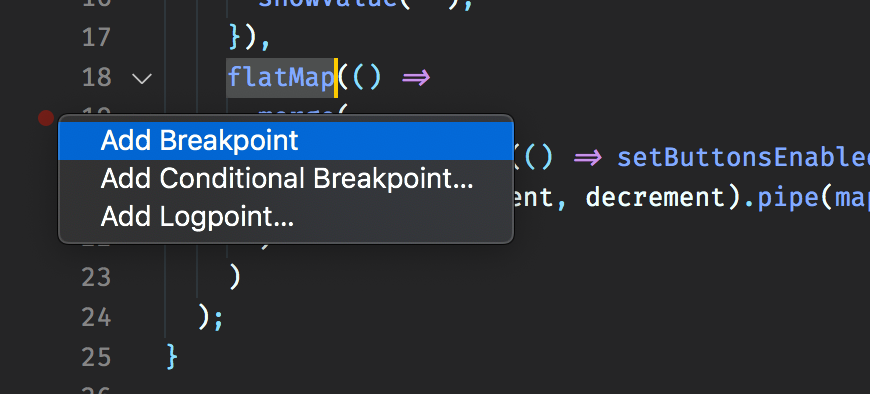
\includegraphics[height=\textheight/2]{figures/add-breakpoint.png}
        \caption{Add a Breakpoint}
    \end{figure}
\end{frame}

\note[itemize] {
    \item How to debug a problem? Well...
    \item Add a breakpoint
    \item Imperative programming debugging
    \item Helps sometimes (lambda functions, ...)
    \item Often useless (stack traces, program step controls...)
    \item What else?
}

\begin{frame}[fragile]{Debugging: The Reality}
    \begin{figure}[H]
        \centering
        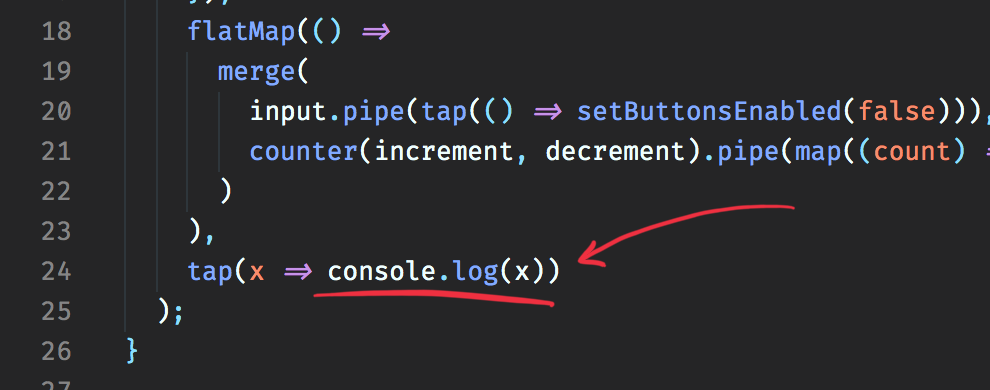
\includegraphics[height=\textheight/2]{figures/consolelog.png}
        \caption{Add Trace Logs}
    \end{figure}
\end{frame}

\note[itemize] {
    \item After some time with RxJS
    \item Stuff gets more complex
    \item Debugging === Trace Logs
    \item Sprinkle log statements throughout the program
    \item Hope to get the right hint
    \item Remove (hopefully) everything again
}

\begin{frame}[fragile]{Debugging: Can this be it?}
    \begin{figure}[H]
        \centering
        
\includegraphics[height=\textheight/2]{figures/person-shrugging_1f937.png}
        \caption{\tiny{Source: \url{https://emojipedia.org/person-shrugging/}}}
    \end{figure}
\end{frame}

\note[itemize] {
    \item Frustration -> Reason Research topic
    \item There are concepts and solutions for RP debugging
    \item Reactive Debugger, Scala \cite{10.1145/2884781.2884815}
    \item Improved logging tools rxjs-spy
    \item Visualizers rxviz, rxjs visualizer
    \item But why does nobody seem to use them?
    \item Why are they not popular?
    \item -> Research Questions
}

\begin{frame}[fragile]{Research Questions}
    \begin{enumerate}
        \vfill\item[RQ1] \textbf{What challenges} do software engineers face when debugging RxJS-based applications?
        \vfill\item[RQ2] How can the \textbf{experience} of software engineers during the debugging process of RxJS-based applications \textbf{be improved}?
        \vfill\item[\color{gray}{RQ3}] \color{gray}{What is the \textbf{impact of proposed solutions} on the debugging experience of software engineers?}
    \end{enumerate}
\end{frame}

\note[itemize] {
    \item First: Collect and Validate information
    \item How do engineers debug RxJS?
    \item What do they like? Dislike?
    \item Validate this data in an observational study
    \item Second: Propose a solution to improve
    \item Third: Implement and validate solution
    \item Not part of this work
    \item Already started with in current iteration
}


\section{Interviews and War Stories}



\begin{frame}[fragile]{Call for ``War Stories''}
    \begin{figure}[H]
        \centering
        
\includegraphics[height=0.6\textheight]{figures/tweet-interview.png}
        \caption{\tiny{Source: \url{https://twitter.com/swissmanu/status/1242429409208029185}}}
    \end{figure}
\end{frame}

\note[itemize] {
    \item First: Collect and Validate information
    \item How do engineers debug RxJS?
    \item What do they like? Dislike?
    \item Validate this data in an observational study
    \item Second: Propose a solution to improve
    \item Third: Implement and validate solution
    \item Not part of this work
    \item Already started with in current iteration
}

\begin{frame}[fragile]{Getting Started with RQ1}
	\begin{vfilleditems}
		\item Talk to practitioners
		\item 1:1 Interviews
		\item Written ``War Story'' Reports
	\end{vfilleditems}
\end{frame}


\begin{frame}{Interviews}
	\begin{vfilleditems}
		\item Informal interviews with five participants
	\end{vfilleditems}
\end{frame}

\begin{frame}{War Stories}
	\begin{vfilleditems}
		\item Request via Twitter and direct emails
		\item Responses from five engineers, including one RxJS core team member
	\end{vfilleditems}
\end{frame}

\begin{frame}{Results}

\end{frame}


\section{Observational Study}
\begin{frame}{Hypothesis}
    If software engineers must solve an RxJS-based problem, then they \textbf{will instrument the code manually} in order to understand its behavior.
\end{frame}

\begin{frame}{Study Design}
    \begin{vfilleditems}
        \item Observational Study
        \item Two Problems
        \item 25 Minutes per Problem
        \item 
    \end{vfilleditems}
\end{frame}

\begin{frame}{Problem Example}

\end{frame}

\begin{frame}{Results}

\end{frame}

\section{Conclusion}
\begin{frame}{}

\end{frame}

\section{Future Work}
\begin{frame}[fragile]{Future Work}
    \begin{vfilleditems}
        \item Manuel Alabor \cite{10.1145/2501654.2501666}
        \item Manuel Alabor
        \item Manuel Alabor
    \end{vfilleditems}
\end{frame}

\begin{frame}[plain, noframenumbering]
  \centering
  \vfill
  {\fontsize{40}{50}\selectfont Q \& A}
  \vfill
\end{frame}

\appendix
\begin{frame}[allowframebreaks]{References}
	\printbibliography
\end{frame}

\end{document}